\documentclass[10pt,conference]{IEEEtran}
%\IEEEoverridecommandlockouts
\usepackage[spanish,es-tabla]{babel}
\usepackage[spanish]{babel}
\renewcommand{\baselinestretch}{1.5}     %interlineado
\usepackage[utf8]{inputenc} 
\usepackage[square,numbers]{natbib}
\bibliographystyle{abbrvnat}
\usepackage{float}                      % para usar [H]
\usepackage{amsmath,amssymb,amsfonts}
\usepackage{graphicx}
\usepackage{textcomp}
\usepackage{xcolor}
\usepackage{ragged2e} % \justify

%---------- encabezado pagina
\usepackage{fancyhdr}
\pagestyle{fancy}
\fancyhf{}
\rhead{\thepage}
\renewcommand{\headrulewidth}{0pt}
%-----------------


%-----------------
\def\BibTeX{{\rm B\kern-.05em{\sc i\kern-.025em b}\kern-.08em
    T\kern-.1667em\lower.7ex\hbox{E}\kern-.125emX}}
%__________

\title{Técnicas de Representación del Conocimiento \\ {\Large Inteligencia Artificial 2}}
%--------------------------------------------
\author{
\IEEEauthorblockN{1\textsuperscript{do} Angely Mendez}
\IEEEauthorblockA{\textit{Escuela de Informática} \\
\textit{Universidad Nacional de Trujillo}\\
Trujillo, Perú \\
t052701020@unitru.edu.pe}
\and
\IEEEauthorblockN{2\textsuperscript{ero} Ciara Mendez}
\IEEEauthorblockA{\textit{Escuela de Informática} \\
\textit{Universidad Nacional de Trujillo}\\
Trujillo, Perú \\
t022700920@unitru.edu.pe}
}

%%--------------------------------------------
\begin{document}
\renewcommand{\IEEEkeywordsname}{{\bfseries Palabras claves:}} % Colocar Keywords en Spanish

\maketitle
%-------------------------------------------
\begin{abstract}
Este documento es una investigación que describe tres  Técnicas de Representación del Conocimiento, las cuales son: Redes Semánticas, Marcos (Frames) y Ontologías. Este articulo es la recopilación de varias investigaciones a nivel nacional e internacional, en los que abordan un problema, describen de manera formal y computacionalmente el dominio sobre el cual se quiere operar, considerando tanto a los objetos como a las relaciones entre ellos combinando estructuras de datos y procedimientos interpretativos que, empleados correctamente hicieron que un programa exhiba
un comportamiento inteligente; respecto a las mencionadas técnicas, se explican sus definiciones y dos investigaciones de cada una, con la finalidad de entender la importancia de las ciencias de la computación en la vida diaria.  
\end{abstract}

\begin{IEEEkeywords}
Representación del conocimiento, Redes Semánticas, Marcos, Ontologías, ciencias de la computación.
\end{IEEEkeywords}

\section{\textbf{Introducción}}
Los seres humanos son buenos para comprender, razonar e interpretar el conocimiento. Y utilizando este conocimiento, pueden realizar diversas acciones en el mundo real. Pero, ¿cómo podemos representar este conocimiento?. 

En inteligencia artificial, el conocimiento se puede representar de varias formas empleando varias técnicas, según la estructura del conocimiento o la perspectiva del diseñador o incluso el tipo de estructura interna utilizada. Una representación efectiva del conocimiento debe ser lo suficientemente rica como para incluir el conocimiento requerido para resolver el problema. Debe ser natural, compacto y mantenible. 

Entonces este informe presenta información al respecto, el cual está organizado de la siguiente manera: en primer lugar, se explican los conceptos teóricos: definiciones de las tres técnicas, luego se da énfasis en dos investigaciones para cada una de ellas y para finalizar las conclusiones más relevantes.
%------------------------------------------
\section{\textbf{Técnicas de Representación del Conocimiento}} 
%\vspace{-22 mm}

\subsection{\underline{\textbf{Redes Semánticas}}}
Están basadas en la idea de que los objetos o los conceptos pueden ser unidos por alguna relación.
Estas relaciones se representan usando una liga que conecte dos conceptos. Los nodos y las ligas pueden ser cualquier cosa, dependiendo de la situación a modelar. \citep{tema4pdf46}. En un grafo o red semántica los elementos semánticos se representan por nodos como se muestra en la Figura ~\ref{R0}.

Elementos de la representación:
\begin{itemize}
    \item Las \textbf{instancias} se representan por constantes.
    \item Las \textbf{clases} se representan por constantes.
    \item Las \textbf{relaciones} clase–superclase se representan por hechos de la forma es un $(> clase>,<super-clase>)$.
    \item Las relaciones instancia–clases se representan por hechos de la forma inst
    $(<instancia>,clase>)$.
    \item Cada propiedad se representa por un predicado binario de la forma
    prop $(<instancia o clase>,<propiedad>,valor>)$.
    \item La constante inicio representa la clase inicial de la jerarquía.
    \item Las propiedades de una instancia es una lista de pares \textbf{atributo–valor}.
\end{itemize}

\begin{figure}[H]
\begin{center}
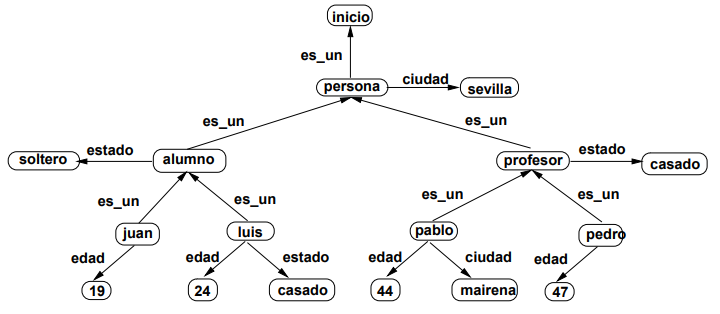
\includegraphics[width=8cm, height=5cm]{figuras/R0.PNG}
\caption{Ejemplo Redes Semánticas- Tomado Universidad de Sevilla, España.}
\label{R0} 
\end{center}
\end{figure}

A continuación, se presentan dos investigaciones donde se evidencia la aplicación de la técnica Redes Semánticas:
\begin{enumerate}
\item En la investigación \textit{\textbf{“Análisis de causas de retraso en proyectos de construcción complejos: un enfoque de análisis de redes semánticas”}}, \citep{zarei2018delay}.

\textbf{\underline{Problema:}} Los retrasos se encuentran entre los adversarios más cruciales para el éxito y el rendimiento de los proyectos de construcción, lo que
hace que el análisis y la gestión de retrasos sean una tarea crítica para los gerentes de proyectos. Esta tarea será muy complicada en proyectos de gran envergadura como la construcción, que suelen consistir en una red compleja de entidades heterogéneas en continua interacción. Los enfoques y métodos tradicionales para el análisis de las demoras y sus causas han sido criticados por su capacidad para manejar proyectos complejos y por considerar las interrelaciones entre las causas de las demoras. 

\textbf{\underline{Resultados:}} Al abordar esta brecha, esta investigación presenta un enfoque alternativo para el análisis de las causas del retraso mediante la adopción del método de análisis de redes semánticas (SNA). El documento informa los resultados de una investigación de retrasos en proyectos de construcción en el sector Petróleo-Gas-Petroquímico usando SNA. Tal como se muestra en la Figura  ~\ref{R1}, las causas pertenecen a los conceptos Group A: Retrasos relacionados con los procesos de contratación, Group B: Retrasos relacionados con las negociaciones iniciales, C: Retrasos relacionados con el proceso de planificación, D: Retrasos relacionados con el proceso de control, donde se examinó y discutió empíricamente la capacidad del método para identificar y clasificar las causas de las demoras, el análisis ayudó a una identificación más precisa del principal factor que causa retrasos en los proyectos de construcción petroquímicos iraníes, las \textit{'deficiencias de las negociaciones iniciales'}, una etapa en la que los puntos de vista y expectativas contradictorias de los diferentes actores ejercen presión sobre el proceso. 

\begin{figure}[H]
\begin{center}
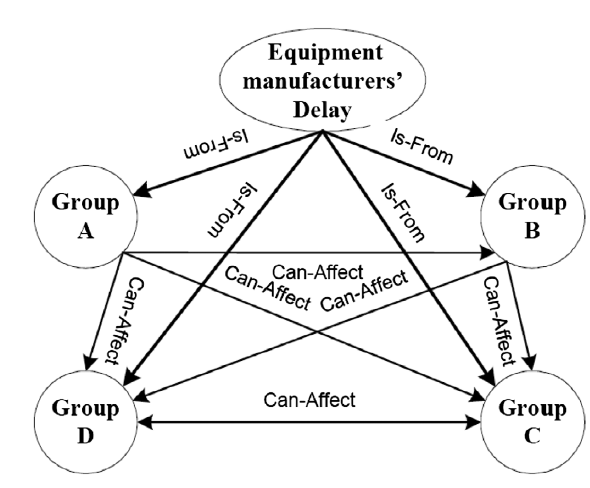
\includegraphics[width=6cm, height=5cm]{figuras/R1.PNG}
\caption{Red semántica de causas de retraso de IPI.}
\label{R1} 
\end{center}
\end{figure}

\textbf{\underline{Importancia:}}  El documento argumenta que el SNA conduce a una \textbf{comprensión más integral} de las principales causas de retraso en proyectos grandes y complejos, lo que permite una mejor identificación y mapeo de las interrelaciones entre estos factores discretos lo que puede ayudar a los gerentes a seleccionar las medidas apropiadas para eliminarlas.


\item Otra investigación es \textit{\textbf{“Aplicación de un método para el análisis de las redes semánticas en pacientes que sufrieron un accidente cerebro vascular”}}, \citep{vivas2010aplicacion}.

\textbf{\underline{Problema:}}
Numerosas investigaciones han estudiado las alteraciones en las relaciones semánticas entre conceptos producidas por diversas patologías, centrándose en su mayoría en pacientes con demencia (Alzheimer en particular) y esquizofrenia y ninguna en accidente Cerebro Vascular (ACV); por ello se presenta esta aplicación de un método de estimación de distancias semánticas, denominado DISTSEM, en pacientes que sufrieron un Accidente Cerebro Vascular (ACV). Este método se basa en la Teoría de Propagación de la Activación,  la cual supone que la memoria semántica se organiza en forma de una red de acuerdo con líneas de similitud semántica. Así, cuantas más propiedades en común haya entre dos conceptos, más cerca se encontrarán en la red.

\textbf{\underline{Resultados:}}
Los resultados ponen de manifiesto que algunos pacientes luego de sufrir un ACV realizan estimaciones de proximidad entre conceptos, distintas a las esperables de acuerdo al desempeño del grupo control. Las respuestas no fueron homogéneas. Se hallaron sujetos que establecieron escasas asociaciones entre los pares de palabras. También se hallaron sujetos que encontraron más vinculaciones que el grupo control, incluso encontrando similitudes en aquellos pares que no tenían vinculación semántica y que utilizaron justificaciones para realizar sus estimaciones, que no se corresponden con categorías semánticas sino que se basan principalmente en la funcionalidad. La lectura de estos resultados a la luz de la Teoría de Propagación de la Activación indica que dichos pacientes tienden a fallar en el proceso de búsqueda dentro de la red, particularmente en la regulación de la propagación de la activación que es necesaria para realizar la tarea.

\begin{figure}[H]
\begin{center}
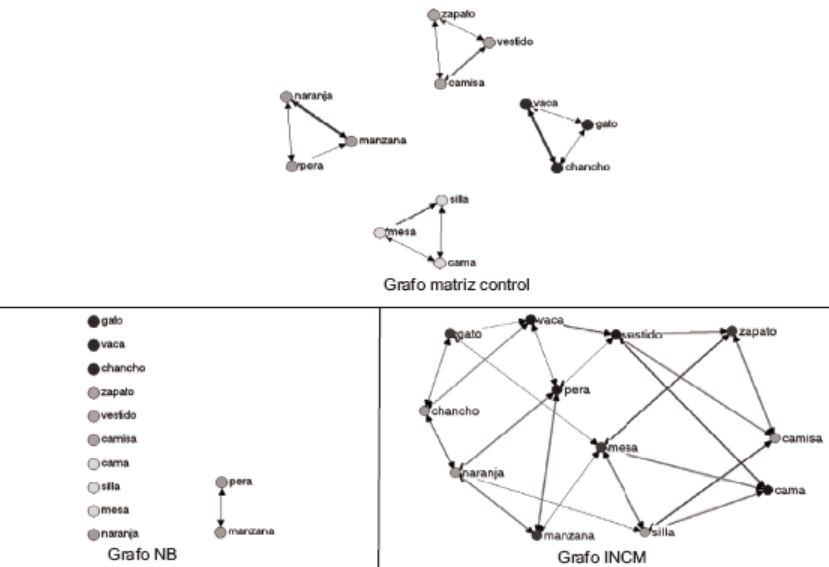
\includegraphics[width=8cm, height=6cm]{figuras/RD22.JPG}
\caption{Grafo Ilustrativo de la Red semántica.}
\label{RD22} 
\end{center}
\end{figure}

\textbf{\underline{Importancia:}}
El método DISTSEM permite capturar una red semántica conformada a partir de las estimaciones de distancias semánticas realizadas por un sujeto en función de un universo
de pares de conceptos presentados por el examinador. Mediante la aplicación del método es posible constituir una matriz semántica, describirla y analizarla. El Método
DISTSEM cuenta con una sistematización informática (Infosem) para hacer más amigable y versátil su utilización en diferentes ámbitos e intereses de investigación. Su principal
desarrollo hasta el momento ha sido en torno a la evaluación educativa.
\end{enumerate} 
%---------------------------------------------------------------------------
\subsection{\underline{\textbf{Marcos (Frames)}}}
Los frames son una estructura en la cual se pueden representar \textbf{valores, restricciones, procesos, atributos, relaciones etc}. Tienen relaciones de pertinencia y herencia, es decir especialización y generalización (por lo que se parecen a la programación orientada a objetos) \citep{21Repres15}.

Elementos de la representación:
\begin{itemize}
    \item Las \textbf{instancias} se representan por constantes.
    \item Las \textbf{clases} se representan por constantes.
    \item Cada \textbf{propiedad} se representa por una igualdad de la forma $<atributo>:<valor>$
    \item Las relaciones clase–superclase se representan por hechos de la forma clase $(<clase>,<sup-clase>,[<prop-1>,..,<prop-n>])$
    \item Las relaciones instancia–clase se representan por hechos de la forma
    instancia $(<clase>,<sup-clase>,[<prop-1>,..,<prop-n>])$
    \item La constante inicio representa la clase inicial de la jerarquía.
    \item Las propiedades de una instancia es una lista de pares \textbf{atributo–valor}.
\end{itemize}

\begin{figure}[H]
\begin{center}
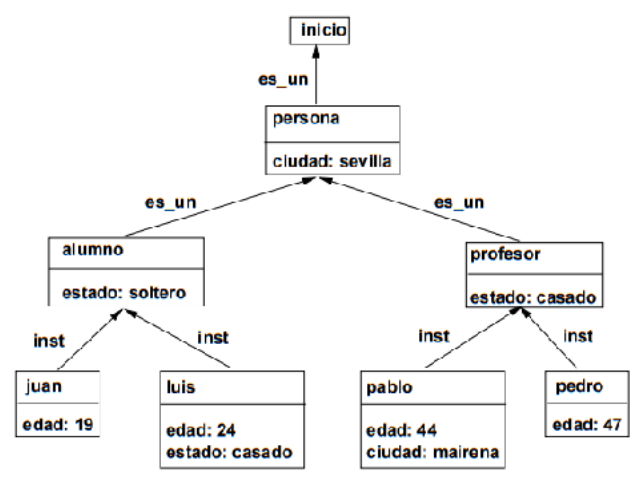
\includegraphics[width=6.5cm, height=4.5cm]{figuras/F1.PNG}
\caption{Ejemplo Representación del Conocimiento (Marcos o Frames) - Universidad Nacional de Tucumán.}
\label{F1} 
\end{center}
\end{figure}

Una de las ideas intuitivas detrás de los Frames, es que la memoria se basa mucho en estereotipos (propiedades típicas de los objetos), tal como se muestra en la Figura ~\ref{F1}.

A continuación, se presentan dos investigaciones donde se evidencia la aplicación de esta técnica:
\begin{enumerate}
\item La investigación \textit{\textbf{“Marcos predicativos asociados al concepto signo y síntoma en textos sobre medicina en español”}}, \citep{lopez2020marcos}.

\textbf{\underline{Problema:}} En la redacción de textos sobre medicina, una precisa selección de verbos facilita la comprensión de terminología y las relaciones conceptuales de este dominio. En este artículo se pretendió extraer verbos que normalmente coocurren con sintagmas nominales que representan el concepto \textbf{signo y síntoma} en textos médicos en español y describir sus patrones. Con una metodología de corpus y la plataforma $Sketch Engine$ se elaboro un inventario de dichos verbos y se organizo semánticamente en un \textbf{esquema de marcos y submarcos}, a los que se han asociado plantillas con información semántica y sintáctica para las predicaciones verbales que incluyen signo y síntoma como argumentos.

\textbf{\underline{Resultados:}} Tras el análisis de patrones y líneas de concordancia y la consulta a un experto médico, se propuso un esquema con siete marcos diferentes para la escena. una persona tiene signos y síntomas, probablemente asociados a una enfermedad, como se muestra en la Figura ~\ref{F2}. Refleja las predicaciones y categorías conceptuales ‘activadas’ en este contexto y sus posiciones en la estructura argumental. Se han seleccionado verbos frecuentes que estaban presentes en todos los subcorpus, recuperados con las fórmulas de búsqueda descritas en el apartado 2.2. Y se han aplicado al proyecto de investigación CombiMed (Léxico Combinatorio en Medicina: cognición, texto y contexto) con vistas a la creación de un inventario de base semántica en español para la redacción y traducción de textos médicos. 

\begin{figure}[H]
\begin{center}
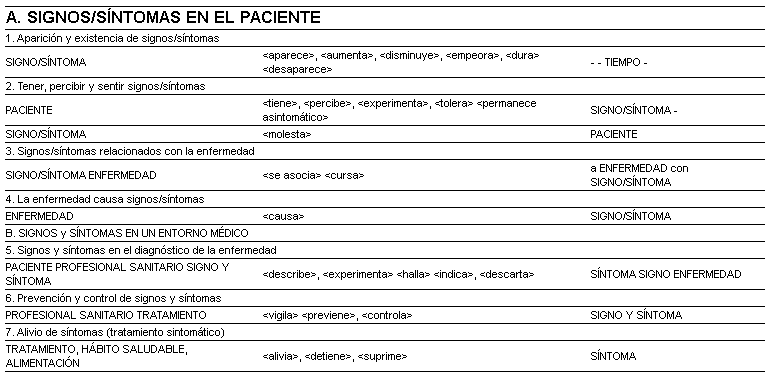
\includegraphics[width=9cm, height=6cm]{figuras/F2.PNG}
\caption{Marcos y submarcos de las predicaciones verbales que incluyen SIGNO Y SÍNTOMA como argumentos.}
\label{F2} 
\end{center}
\end{figure}

\textbf{\underline{Importancia:}} En estudios previos se ha señalado la importancia de patrones léxico-sintácticos de verbos en el lenguaje especializado. Con lo que se espera que la representación de estos marcos predicativos en español beneficie a científicos, redactores técnicos y traductores que comunican avances científicos en lengua española, y por ende, al público lego para una mayor comprensión respecto a signo y síntoma.

\item Otra investigación es \textit{\textbf{“Tierra común, Marcos y Ranuras para la comprensión en Sistemas de Diálogo”}}, \citep{blache2021common}

\textbf{\underline{Problema:}} Este artículo presenta un sistema de diálogo para capacitar a los médicos para dar malas noticias. La originalidad de este trabajo radica en su representación del conocimiento. Toda la información conocida antes del diálogo (el universo del discurso, el contexto, el escenario del diálogo) así como el conocimiento transferido del médico al paciente durante la conversación se representa en una estructura de conocimiento compartido denominada terreno común, que constituye el núcleo del sistema.

\textbf{\underline{Resultados:}}
Centrándose en dos aspectos: la representación del conocimiento para comprender y generar comportamientos del paciente. Formalmente, el terreno común está formado por un conjunto de tramas, que reúnen información, denominada ranuras, como se ilustra en la Figura ~\ref{F3}. Un valor de ranura puede ser atómico (por ejemplo, Nombre, Edad, etc.) o (por ejemplo , Persona, Patología). Cada espacio es ponderado, en escala: obligatorio, importante, opcional. Y una información puede depender de otro marco. Por ejemplo, el médico no puede describir ninguna remediación antes de haber presentado la patología.

\textbf{\underline{Importancia:}}
El uso de técnicas de diálogo para capacitar a los médicos representa un caso de uso fundamental
tanto en la perspectiva de desarrollar nuevas técnicas de diálogo como en términos de aplicación. La representación basada en marcos ofrece primero la posibilidad de utilizar técnicas de clasificación que identifiquen directamente el marco que se va a instanciar. Gracias a ello se propuso un método original de llenado de ranuras, basado en la información de terreno común y semántica distribucional. La generación de las reacciones del agente y su adaptación al discurso del médico aprovecha directamente la representación.

\begin{figure}[H]
\begin{center}
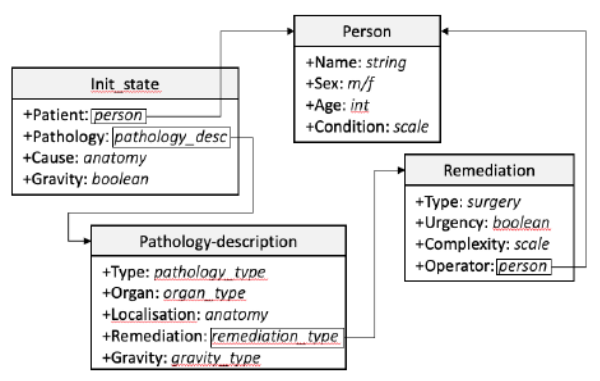
\includegraphics[width=7cm, height=5cm]{figuras/F3.PNG}
\caption{Ejemplo de marcos y ranuras utilizados en la investigación.}
\label{F3} 
\end{center}
\end{figure}



\end{enumerate}

%---------------------------------------------------------------------------
\subsection{\underline{\textbf{Ontologías}}}
 Las ontologías son herramientas útiles para la comunicación entre expertos en un área determinada. Se puede formalizar conceptos en un dominio para que luego sean validadas por computadores y obtener respuestas más favorables a la hora de
consultarlas. \citep{gree} \par
Formalmente las ontologías son usadas para representar el conocimiento, la razón por la cual se usan estos esquemas, es debido a que nos permite realizar búsquedas de información con carácter semántico, con la finalidad de obtener resultados mucho más óptimos. \citep{melgar2011modelo} \par
Una búsqueda semántica se puede definir como un proceso de optimización de los resultados obtenidos por un motor de búsqueda, utilizando las propiedades de la semántica. En este contexto, las ontologías nos ofrecen mecanismos de relación conceptual que nos permiten transformar la consulta en una más enriquecida y representada de manera estructurada, para luego compararla con la ontología que maneja el motor utilizado y así devolver mejores resultados \citep{rujiang2009improving} \par
Para la representación de ontologías se utilizan diferentes lenguajes que han ido evolucionando en el tiempo, la finalidad de estos lenguajes es de representar a las mismas de manera que sean entendibles por el computador y por el usuario, por ejemplo: RDF/XML y OWL y entornos como Protege. (Ver Figura  ~\ref{fO1}.)

\begin{figure}[H]
 \begin{center}
       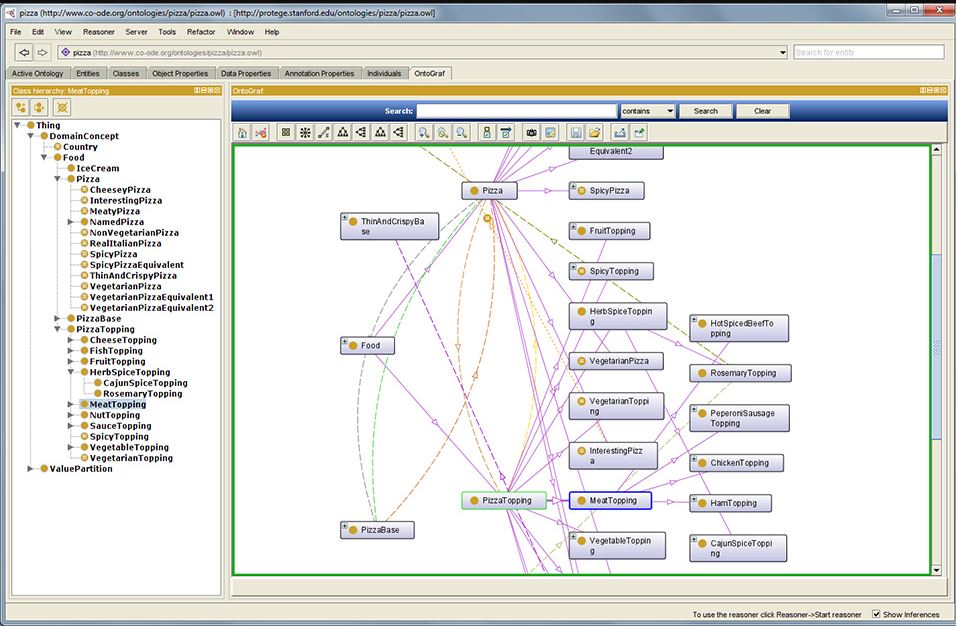
\includegraphics[width=7cm, height=4cm]{figuras/O1.JPG}
      \caption{Ejemplo de ontología en Protegé http://protege.stanford.edu/}
      \label{fO1} 
      \end{center}
\end{figure}

\par A continuación, dos investigaciones respecto a la técnica de representación del conocimiento de ontologías :
\begin{enumerate}
\item En la tesis \textbf{\textit{“Diseño de un modelo para la Recuperación de Documentos basado en Ontologías en el Dominio de la Ingeniería Informática”}} \citep{gomez2014}, se propusó el uso de ontologías como estructura básica para la representación del conocimiento por su eficacia en realizar la recuperación de documentos. Además, se planteó utilizar un proceso de etiquetación semántica de documentos para relacionar cada documento digital con - al menos - una entidad de la ontología con la finalidad de poder realizar búsquedas mediante el uso de etiquetas y lenguaje natural.  (Ver Figura ~\ref{fO2})

\begin{figure}[H]
 \begin{center}
       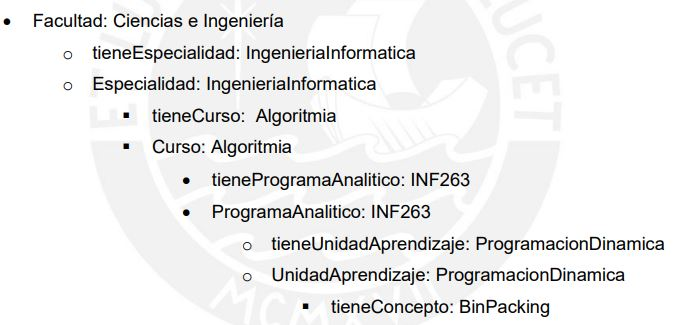
\includegraphics[width=6cm, height=3cm]{figuras/O2.JPG}
      \caption{Un ejemplo de hechos sacado de la ontología.}
      \label{fO2} 
      \end{center}
\end{figure}
%\vspace{-43 mm}
\textbf{\underline{Problema:}}
En la especialidad de Ingeniería Informática de la PUCP existe la necesidad en los estudiantes de buscar documentos que contengan información sobre los cursos de la carrera.(ámbito o dominio del que se habla es bastante amplio).
Actualmente, se cuenta con repositorios digitales de documentos, que almacenan imágenes escaneadas o documentos en formato PDF, a la que los alumnos y profesores tienen acceso. Sin embargo, actualmente estos documentos no proporcionan alguna manera de reconocer su contenido y, así, facilitar su recuperación. \par
\textbf{\underline{Importancia:}}
Ante ello se presentó el análisis del dominio de Ingeniería Informática, para proponer una estructura ontológica capaz de soportar y almacenar todas las relaciones e inferencias producidas en el dominio. (Ver Figura ~\ref{fO3}) \par

\begin{figure}[H]
 \begin{center}
       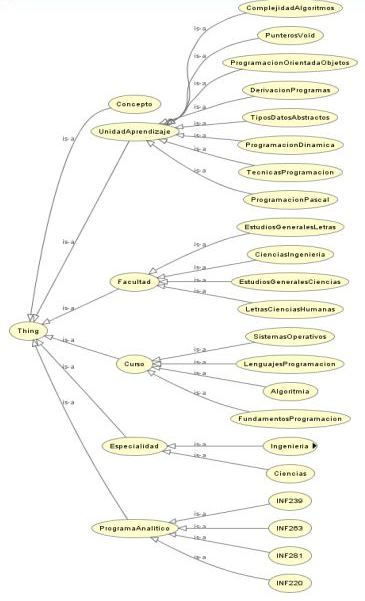
\includegraphics[width=6cm, height=10cm]{figuras/O3.JPG}
      \caption{Ontología planteada en el dominio de la Ingeniería Informática.}
      \label{fO3} 
      \end{center}
\end{figure}
\textbf{\underline{Resultados:}}
En el análisis del dominio, se establecieron una serie de restricciones a medida que se fue desarrollando la ontología, esto con la finalidad de reducir incongruencias. Luego de probar el aplicativo, se observó que el modelo planteado cubre en gran medida las necesidades planteadas. Aun no se puede cumplir con realizar consultas en lenguaje natural. Debido a que el procedimiento de análisis se propuso, a manera que, limitemos al usuario a utilizar consultas que directamente sean entidades de la ontología en la estructura.

\item En el artículo de investigación titulado \textbf{\textit{“Seguridad informática de un sistema basado en ontología de control vía Web de dispositivos domóticos”}} \citep{huiman2016seguridad}.

\begin{figure}[H]
 \begin{center}
       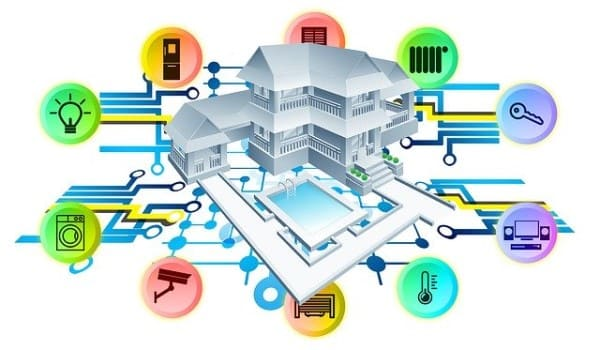
\includegraphics[width=8cm, height=5cm]{figuras/O4.JPG}
      \caption{Estructura de sistema domótico.}
      \label{fO4} 
      \end{center}
\end{figure}

Los sistemas domóticos(Ver Figura ~\ref{fO4}) son un conjunto de sistemas de automatización de una vivienda con fines de gestión energética, seguridad, bienestar y comunicación; integrados por controladores, actuadores y sensores, pudiendo ser gestionados remotamente desde un servidor web, tal y como lo afirman García Sánchez y Moreno Martín (2013, p. 8), y mediante una ontología.

\begin{figure}[H]
 \begin{center}
       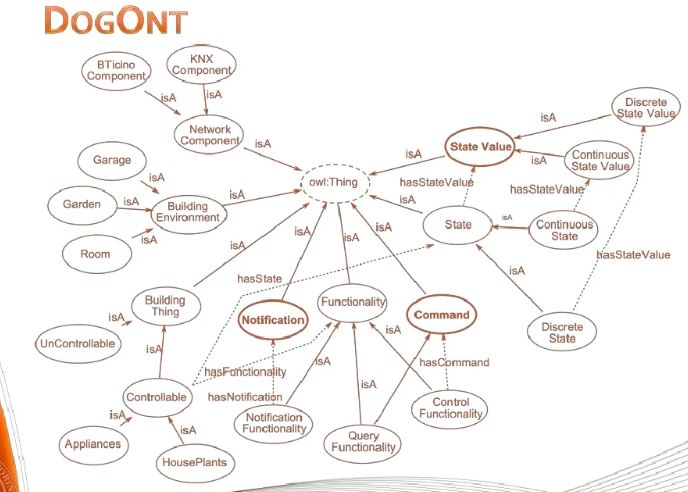
\includegraphics[width=7cm, height=4cm]{figuras/O7.JPG}
      \caption{Ejemplo de sistema domótico.}
      \label{fO7} 
      \end{center}
\end{figure}
\textbf{\underline{Importancia:}}
Las ontologías son componentes de la Web semántica que, implementan conceptos relacionados, razonamiento y reglas de inferencia en la Web . Un ejemplo es DogOnt (Ver Figura ~\ref{fO7}) desarrollada como una ontología que representa conceptos de ambientes y dispositivos referidos a una vivienda domótica, de manera remota desde un servidor web y, en una configuración adecuada, reducir el consumo de energía de múltiples viviendas, teniendo en cuenta la reutilización de componentes ante usuarios concurrentes en un mismo ambiente con actividades parecidas o priorizables.\par
\textbf{\underline{Problema:}}
Sin embargo, la complejidad inherente al desarrollo de aplicaciones web de hoy, como las basadas en ontologías que controlarían remotamente a los sistemas domóticos en viviendas automatizadas, trae consigo una falla en la seguridad informática, vulnerabilidad que es propia de la Web semántica ya que los ataques informáticos, en un futuro próximo, se centrarán en modificar el significado de conceptos incluidos en una ontología de la Web semántica para permitir la intrusión en los sistemas, por ejemplo, de automatización de vivienda. 

\begin{figure}[H]
 \begin{center}
       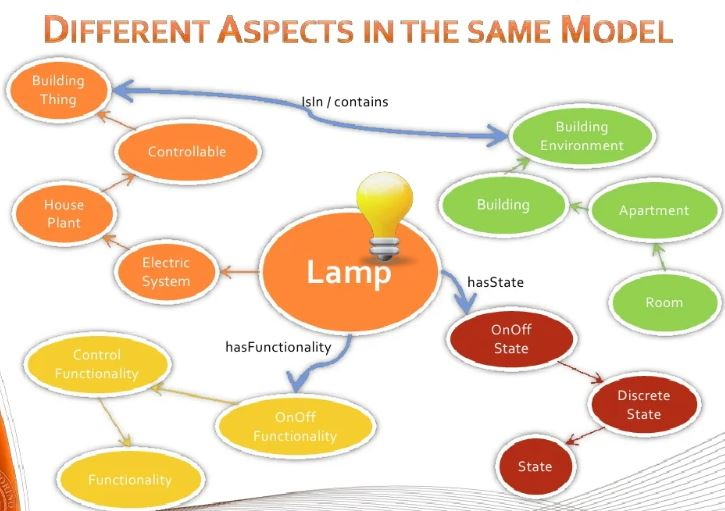
\includegraphics[width=7cm, height=4cm]{figuras/O8.JPG}
      \caption{Ontología en DogOnt.}
      \label{fO8} 
      \end{center}
\end{figure}
\textbf{\underline{Resultados:}}
Por eso se concluyó que, para mitigar el riesgo informático de una ontología controladora de sistemas domóticos de manera remota expuesta desde un servidor web, es necesario un criptosistema simétrico basado en el lenguaje XML Encryption con el Advanced Encryption Standard con un marco de desarrollo y ECC Mixed Coordinates Cryptography para encriptar el mensaje apoyándose en OWL / OWL-S, debido a su capacidad de asegurar, mediante clases privadas, las reglas de inferencia y consultas en lenguaje plano que intercambian el servidor web con el controlador central del sistema domótico.

\begin{figure}[H]
 \begin{center}
       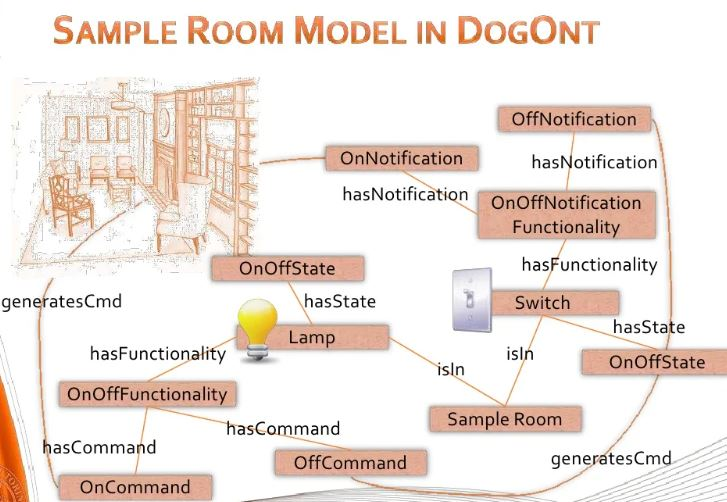
\includegraphics[width=8cm, height=5cm]{figuras/O9.JPG}
      \caption{Ejemplo de sistema domótico en una habitación usando herramienta de desarrollo de Ontología DogOnt.}
      \label{fO9} 
      \end{center}
\end{figure}

\end{enumerate}

%---------------------------------------------------------------------------

%---------------------------------------------------------------------------
\section{\textbf{Conclusiones}}

Este informe presentó información relevante acerca de tres técnicas de Representación del Conocimiento empleados en la Inteligencia Artificial, explicándose también los conceptos teóricos relacionados a ellas. Además de permitir conocer sobre algunas investigaciones que se vienen realizando año a año, entendiendo las diversas aplicaciones en la vida diaria. Concluimos que la mayoría analiza la problemática y dependiendo de sus características se establecieron los procesos así como la técnica a emplear, para representar información o conocimiento del mundo real en una forma que se pueda entender y usar para resolver problemas de la vida real. Finalmente, las investigaciones expuestas en este trabajo de recopilación, sirven como antecedentes y base a futuros investigadores a nivel nacional e internacional, que pueden ser usados tanto en el área comercial o académico.
%-------------------------------------------------------
\medskip
\bibliography{refer}
\end{document}